%!TEX root = ../thesis.tex

\section{Algorithm implementation}\label{section:implementation}

\todo[inline]{Add introduction}

\subsection{Language choices}\label{section:language-choices}

Bioinformatics datasets sizes severely impact the computational time of algorithms, therefore limiting the choice of programming language one can make when designing a program.
Character evolution instances are in no way comparable to genomic sequences; still, the amount of data is not trivial, and using a low-level language might be preferred.

Even though C can be considered as the go-to compiled language for fast computations, \cc{} keeps up in speed really well \cite{PLB2008}, while providing a series of types of abstractions.
Moreover, \cc{} can be complemented by powerful libraries like \href{http://www.boost.org/}{Boost}, which can improve development speed by a decent margin.

The \cc{}14 Standard has been supported by GCC since 2015, with the release of GCC 5.
Admittedly, most of the language features we used belong to \cc{}11, but we decided to write cleaner code with the help of brace-enclosed initializer lists.

Scripting languages were used to test the correctness of our implementation throughout the developing process.
Heavy use of the Bash scripting language is to be expected when developing on a Unix system, however, for more complex tasks (like working on matrices), we believe Python to be a more fitting candidate.
In fact, we implemented a Python script to check whether a c-reduction is successful for a given PPP instance.

\todo[inline]{Talk about stdc++ in more detail?}

\subsubsection{Boost libraries}\label{section:boost-libs}

The Boost libraries provide generic implementations for concepts and abstractions not yet present in the Standard Library, in fact, as of now, ten Boost libraries are included in the \cc{}11 Standard.

\todo[inline]{Talk about CXX11 ABI?}

By default, GCC compiles with no optimization ($-O0$), however, Boost advises the use of the $-O2$ or $-O3$ flags. We couldn't notice any problem with compiler optimizations, so we chose $-O3$ as the default flag.

Benchmarking goes a long way to show how much optimization flags influence the performance of our program.

\begin{center}
  \begin{tabular}{c | c c c c c}
    $Instance$ & $-O0$     & $-O1$    & $-O2$    & $-O3$    & $-Ofast$ \\
    \hline
    Instance 0 & $393.43s$ & $33.95s$ & $32.64s$ & $32.55s$ & $32.59s$ \\
    Instance 1 & $579.11s$ & $47.92s$ & $45.56s$ & $44.70s$ & $44.94s$ \\
    Instance 2 & $205.25s$ & $18.68s$ & $17.95s$ & $18.09s$ & $17.80s$
  \end{tabular}
\end{center}

We opted for using Boost wherever the Standard Library didn't provide a reasonable solution to our problems.
Follows the list of libraries and their use-cases in our implementation.

\subsubsection*{Boost Graph}

We based our work on the Boost Graph Library (BGL), which provides a full set of graph operations, algorithms and data structures.
Both the Red-black graph and the Hasse diagram have been implemented using the !boost::adjacency_list! class.

We wrote specialized functions for red-black graph operations like adding and removing vertices to support unique vertex names and species and character vertices counter variables.

While a function for removing edges on a condition is present in the BGL, we needed to implement our own !remove_vertex_if!.
A  use-case for this might be a function which, given a predicate !if_singleton!, removes a vertex if it is a isolated in the graph.

The !boost::print_graph! function doesn't support bundled properties, for this reason we implemented a function overloading the Output stream operator.
Further down the line we made sure the output was sorted correctly to make debugging easier.

\subsubsection*{Boost Bimap}

To provide constant-time access to red-black graph vertices by using their name instead of the underlying identifier we opted for instantiating a bidirectional map between vertices and names (strings).

Recently, we have been evaluating the possibility of using the standard !std::map! instead, with possible rewrites of parts of the current implementation.
Either way, functions for building, accessing and copying the map from the graph were implemented and can be easily adapted to support the choice of map class.

\subsubsection*{Boost Program Options}

While GNU !getopt! is widely used in Bash, C and \cc{} programs, using a Boost library to parse command line arguments is not uncommon when the codebase already includes other Boost header files.
Moreover, Boost Program Options is cross-platform and easy to use, apart from the peculiar syntax for declaring options.

\subsubsection*{Boost Python}

Embedding Python in \cc{} is rather slow and cumbersome.
During development, we found ourselves wanting to make sure the output of our program was a successful c-reduction for the instance in input.
We took this opportunity to learn how to work with Boost Python, embedding a Python interpreter, calling a function from a Python script and then processing its output.
This helped us identify false positives and pinpoint errors in our implementation of the algorithm.

\subsection{Program options}\label{section:program-options}

The software we built supports the use of a set of command-line arguments mainly focused around development testing and debugging.
The program calculates a successful c-reduction for the matrix(ces) in the input FILE(s), if it exists. Usage:

\begin{lstlisting}
  ppp [OPTION...] FILE...
\end{lstlisting}

!OPTION...! is the (optional) list of options given to the program. !--help! stops the execution.
!FILE...! is the list of files given in input; each file must be structured as such:

\begin{itemize}
  \item The first line must contain the size of the matrix (space-separated integers).

  \item Subsequent lines represent the matrix itself.

  \item Empty lines following the first line are ignored.
\end{itemize}

\begin{lstlisting}[aboveskip=0pt]
  $N$ $M$

  $N \times M$ matrix made up of space-separated boolean values
\end{lstlisting}

Follows the list of program options.

\subsubsection*{Help message}

\begin{lstlisting}[aboveskip=\smallskipamount]
  -h, --help
\end{lstlisting}

Display the program usage, description and options.

\subsubsection*{Verbose mode}

\begin{lstlisting}[aboveskip=\smallskipamount]
  -v, --verbose
\end{lstlisting}

\begin{lstlisting}[style=c++_block, aboveskip=\smallskipamount]
  namespace logging {
    extern bool enabled;
  };
\end{lstlisting}

Print information on the operations performed by the program at runtime.

We declare global namespaced variables in a file !globals.hpp!; including the variable introduced in the snippet above.
Variables declared in this file are used throughout the other files. Variables that are not included in our description, however, are only used in the main function of the program, which resides in !main.cpp!.

\subsubsection*{Test with Python script}

\begin{lstlisting}[aboveskip=\smallskipamount]
  -t, --testpy
\end{lstlisting}

Check whether the c-reduction given in output by the algorithm (reduce function) is successful for the instance in input; we accomplish this by calling the python script !check_reduction.py!.

This should only be used for debugging purposes.

\subsubsection*{Exponential version of the algorithm}

\begin{lstlisting}[aboveskip=\smallskipamount]
  -x, --exponential
                         Mutually exclusive with --interactive
                           Mutually exclusive with --nthsource
\end{lstlisting}

\begin{lstlisting}[style=c++_block, aboveskip=\smallskipamount]
  namespace exponential {
    extern bool enabled;
  };
\end{lstlisting}

Test every possible combination of safe sources.

The Find-initial-state procedure is design to produce a safe source in polynomial time, if it exists in the Hasse diagram.
However, we extended the functionality of Find-initial-state to output a list of safe sources when the exponential option is enabled; this makes it possible to realize different safe sources and obtain different c-reductions.

\subsubsection*{User input driven execution}

\begin{lstlisting}[aboveskip=\smallskipamount]
  -i, --interactive
                         Mutually exclusive with --exponential
                           Mutually exclusive with --nthsource
\end{lstlisting}

\begin{lstlisting}[style=c++_block, aboveskip=\smallskipamount]
  namespace interactive {
    extern bool enabled;
  };
\end{lstlisting}

Let the user select, with an interactive menu, which safe source to realize (if the number of safe sources is greater than one).

Whenever the algorithm considers two or more sources to be safe in the Hasse diagram, the program presents a selection of safe sources to the user.

For example, one way to consistently select the second safe source by using the interactive option would be:

\begin{lstlisting}
  while true; do echo 1; done | ppp input_file -i
\end{lstlisting}

\subsubsection*{Maximal subgraph}

\begin{lstlisting}[aboveskip=\smallskipamount]
  -m, --maximal
\end{lstlisting}

Apply the Reduce function to the maximal subgraph \grbcm{} instead of the full graph \grb{}. This is done by calculating a maximal reducible graph before running the algorithm.

Removing minimal characters from the graph simplifies the selection of safe sources (Find-initial-state).

\subsubsection*{\boldmath{$N$}th safe source selection}

\begin{lstlisting}[aboveskip=\smallskipamount]
  -n $n$, --nthsource $n$
                         Mutually exclusive with --exponential
                         Mutually exclusive with --interactive
\end{lstlisting}

\begin{lstlisting}[style=c++_block, aboveskip=\smallskipamount]
  namespace nthsource {
    extern size_t index;
  };
\end{lstlisting}

Select the $n$th safe source whenever the algorithm considers two or more sources to be safe in the Hasse diagram.

When this option is omitted, the default value is 0, which doesn't alter the execution of the program in any way.
However, when the option is defined, the algorithm automatically selects the $n$th safe source to realize, as opposed to the interactive option, which waits for user input.

When the value specified is greater than the number of safe sources available, the last safe source is select.

This option can be considered an alternative to !--interactive!.

\subsection{Boost Graph classes}\label{section:graph-classes}

\lstset{style=c++_block}

Using the !boost::adjacency_list! class is standard procedure when operating with the BGL.

\begin{lstlisting}[style=code_block, basicstyle=\footnotesize\ttfamily\bfseries\color{block_fg}]
  adjacency_list<OutEdgeList, VertexList, Directed,
                 VertexProperties, EdgeProperties,
                 GraphProperties, EdgeList>
\end{lstlisting}

The class models an adjacency list data structure which can be configured with the template parameters VertexList, OutEdgeList and EdgeList; these parameters control which containers are used to store the set of vertices and the set of edges.
Choosing a container over another effectively changes the time complexity of the operations that can be performed on the graph, while also affecting iterator stability.

The template parameter Directed denotes whether the edges in the graph are directed, undirected or bidirectional.

Furthermore, the class offers template parameters for vertex, edge and graph properties. These properties can then be manipulated in the code via property maps or member access operators.

We defined two graph classes which specialize the provided template parameters.

\subsubsection{RBGraph class}\label{section:rbgraph-class}

The red-black graph class implements an undirected bipartite graph with colored edges.
\wip{Continue}

\subsubsection*{Traits and properties}

\todo[inline]{Add introduction?}

\begin{lstlisting}[belowskip=0pt]
  typedef boost::adjacency_list<
    boost::slistS       // OutEdgeList
    boost::listS,       // VertexList
    boost::undirectedS, // Directed
    RBVertexProperties, // VertexProperties
    RBEdgeProperties,   // EdgeProperties
    RBGraphProperties   // GraphProperties
  > RBGraph;
\end{lstlisting}

\paragraph{OutEdgeList}

Set to !boost::slistS!, which proved to be way faster than !setS! (for obvious reasons, !setS! enforces the absence of parallel edges) and slightly faster than !listS!.
Finally, we didn't consider !vecS! to be fitting to our project, since edge removal affects iterator stability and invalidates edge descriptors.

Here's a small benchmark comparing runtimes of the program given in input three different $320 \times 320$ PPP instances:

\begin{center}
  \begin{tabular}{c | c c c}
    $Instance$ & $setS$   & $listS$  & $slistS$ \\
    \hline
    Instance 0 & $17.46s$ & $14.19s$ & $13.05s$ \\
    Instance 1 & $54.15s$ & $44.08s$ & $41.88s$ \\
    Instance 2 & $58.82s$ & $48.31s$ & $45.51s$
  \end{tabular}
\end{center}

\paragraph{VertexList}

Set to !boost::listS!, without much choice, since it provides iterator stability and non invalidable vertex descriptors.
We could not use !slistS! seeing that our implementation of the !maximal_characters! function makes calls to !operator--(int)! on the iterator.

\paragraph{Directed}

Set to !boost::undirectedS! since the graph must be, in fact, undirected.

\paragraph{VertexProperties}

Set to !RBVertexProperties!, which is defined as follows:

\begin{lstlisting}[moreemph={Type}]
  struct RBVertexProperties {
    std::string name;
    Type type;
  };
\end{lstlisting}

We identify each vertex either by its vertex descriptor or using its name, which we enforce to be unique among all vertices (we'll get to how later).

The BGL doesn't support bipartite graphs with its default classes, for this reason we assigned to each vertex a !Type!, which labels the vertex as a species or a character.

\begin{lstlisting}
  enum class Type : bool {
    species,
    character
  };
\end{lstlisting}

As shown in the snippet of code above, !Type! is a scoped enumeration type whose underlying type is !bool!, that \emph{should be} stored as 1 byte (!sizeof(bool)! is implementation-defined).

By storing scoped enumeration types as booleans instead of chars (which are always stored as 1 byte) we noticed a slight reduction in section sizes (compiled binary), while also gaining up to 1 second in speed.

Output of the GNU !size! command:

\begin{center}
  \begin{tabular}{c | c c c c c}
    $Type$ & $text$ & $data$ & $bss$ & $dec$  & $hex$ \\
    \hline
    char   & 291280 & 6824   & 1008  & 299112 & 49068 \\
    bool   & 291192 & 6824   & 1008  & 299024 & 49010
  \end{tabular}
\end{center}

This, however, would most likely not be true when !sizeof(bool)! isn't equal to 1.

\paragraph{EdgeProperties}

Set to !RBEdgeProperties!, which is defined as follows:

\begin{lstlisting}[moreemph={Color}]
  struct RBEdgeProperties {
    Color color;
  };
\end{lstlisting}

Edges in the red-black graph are labeled by a color, which can be either red or black. By default all edges are black (e.g., the initial \grb{}).

Below, we provide the code for the color enumeration type.

\begin{lstlisting}[belowskip=0pt]
  enum class Color : bool {
    black,
    red
  };
\end{lstlisting}

\paragraph{GraphProperties}

Set to !RBGraphProperties!, which is defined as follows:

\begin{lstlisting}[moreemph={RBVertexBimap}]
  struct RBGraphProperties {
    size_t num_species;
    size_t num_characters;

    RBVertexBimap bimap;
  };
\end{lstlisting}

The graph properties store information about the graph; the number of species and characters are kept up to date by overloading and specializing the !add_vertex! and !remove_vertex! functions provided by the BGL.

The same is true for the bidirectional map !bimap!, which stores pairs of vertices and vertex names to enforce uniqueness within the vertex set, and enables constant-time access to a vertex given its name and viceversa.

Finally, the (slightly simplified) definition of the !RBVertexBimap! container is shown in the snippet below.

\begin{lstlisting}[belowskip=0pt, moreemph={RBVertex}]
  typedef boost::bimap<
    boost::bimaps::unordered_set_of<std::string>,
    boost::bimaps::unordered_set_of<RBVertex>
  > RBVertexBimap;
\end{lstlisting}

\subsubsection*{General purpose functions}

The properties of a red-black graph must reflect what lies inside it; operations that modify the structure of a graph, in particular its set of vertices, should not invalidate its properties.
Hence the overloaded functions for adding and removing vertices in the graph.

Below, an example for an overloaded !remove_vertex! function.

\begin{lstlisting}[moreemph={RBVertex, RBGraph},
                   moreemph={[2] remove_vertex}]
  void remove_vertex(const RBVertex v, RBGraph& g) {
    if (is_species(v, g))
      num_species(g)--;
    else
      num_characters(g)--;

    // delete v from the bimap
    bimap(g).left.erase(g[v].name);

    boost::remove_vertex(v, g);
  }
\end{lstlisting}

The function overload for the output stream operator we implemented prints the sorted adjacency lists of each vertex in the graph, with red-black edge support.

The graph \grb{} of figures \ref{figure:1:b} and \ref{figure:3:a}, printed with the ostream operator:

\begin{lstlisting}[keywordstyle=\color{block_fg}]
  s0: --- c1; --- c2; --- c3;
  s1: --- c3;
  s2: --- c0; --- c1;
  s3: --- c0; --- c2;
  c0: --- s2; --- s3;
  c1: --- s0; --- s2;
  c2: --- s0; --- s3;
  c3: --- s0; --- s1;
\end{lstlisting}

When running the program, a function to read the matrix from the file in input is called; this function, !read_graph!, makes sure the file is correctly structured and contains a valid binary matrix whose size must match the one indicated in first line of the file.
Each error in the file is reported with an exception describing what went wrong in the parsing process.

For a $n \times m$ matrix, the vertices inserted in the corresponding red-black graph \grb{} are labeled as \species[0], \dots, \species[n-1] and \character[0], \dots, \character[m-1], depending on whether the vertices represent species or characters; then, the assigned vertex names assigned match those of the definitions used throughout the previous sections.

\subsubsection*{Algorithm functions}

\todo[inline]{Add introduction?}

\paragraph{Active characters}

Following the definitions of active and inactive characters given in section \ref{section:grb}, we implemented two functions to test the state of a character: !is_active! and !is_inactive!.

The choice of implementing two separate functions, instead of a simple check on red edges, falls on wanting to enforce a series of things.
First of all, a vertex can be either active or inactive if and only if it represents a character in \grb{}; in our implementation, a species is neither active nor inactive.
Moreover, we make sure that an active character is incident only on red edges, while an inactive character is incident only on black edges.
Finally, the vertices adjacent to a character must all be species for a character to be considered active or inactive.

\paragraph{Isolated characters}

The !remove_singletons! function was implemented as a loop over each vertex of \grb{}, calling !remove_vertex_if! with a predicate (functor that evaluates to a boolean value) that tests whether a vertex is isolated in \grb{} as argument.

\paragraph{Free and universal characters}

Free and universal characters can be detected by computing the connected components of \grb{} and verifying if a character is connected to all the species in its component.
We are experimenting with ways to simplify this function and extract the connected components computation from it.

\paragraph{Connected components}

To make it so we could apply the !Reduce! procedure to each connected component of the graph we implemented a function that builds the subgraphs of \grb{}, where each subgraph is a copy of the respective connected component.

A subgraph $\grb{}_{0}$ is a !unique_ptr! pointing to a red-black graph whose set of vertices and edges are copied from the \nth{0} connected component.
The output of the function is a !RBGraphVector!, defined as:

\begin{lstlisting}[moreemph={RBGraph}]
  typedef std::vector<std::unique_ptr<RBGraph>> RBGraphVector;
\end{lstlisting}

If the graph \grb{} is connected, the !RBGraphVector! in output will be of size 1, but the !unique_ptr! will be empty.
This is because the purpose of the functions is to build the subgraphs, not copy the whole graph when it isn't needed.

\paragraph{Maximal characters}

Our approach to calculating the maximal characters of a red-black graph involves iterating over each inactive character $\character[i] \in \grb{}$, in any order, and testing it against the characters already in \cm{} (which we will identify as \character[j]).

There are multiple scenarios:

\begin{enumerate}[label=\textbf{S.\arabic*}, ref=S.\arabic*]
  \item \label{enum:maximal:1} the character \character[i] is included in a character $\character[j] \in \cm{}$.

  \item \label{enum:maximal:2} the character \character[i] is not included in any character $\character[j] \in \cm{}$.
  \begin{enumerate}
    \item \label{enum:maximal:2:b} \character[i] includes a character $\character[j] \in \cm{}$.

    \item \label{enum:maximal:2:a} \character[i] overlaps with a character $\character[j] \in \cm{}$.
  \end{enumerate}
\end{enumerate}

Clearly, \ref{enum:maximal:1} describes a scenario where \character[i] is not a maximal character in \grb{}. Conversely, \ref{enum:maximal:2} describes two scenarios where the character \character[i] is maximal in \grb{}.

When \character[i] includes a character $\character[j] \in \cm{}$, i.e., $S(\character[i]) \supseteq S(\character[j])$, we must replace \character[j] with \character[i] in \cm{}.
However, we can't possibly know whether \character[j] was the only character in \cm{} that is included in \character[i] or not; for this reason we keep iterating on the list \cm{} to find other characters that can be removed from it.

Notice how, even if \character[i] overlaps with another character $\character[j] \in \cm{}$, we always need to make sure that \character[i] is not included in any other character of \cm{}, otherwise we fall back into scenario \ref{enum:maximal:1}.

We provide an example of the process in figure \ref{figure:5}.

\paragraph{Maximal reducible graph}

Building a maximal reducible graph \grbcm{} from \grb{} given \cm{} is rather trivial.

To preserve the original \grb{} we first make a copy of it; then, the !bimap! of the copied graph needs to be rebuilt.
This is because the vertex descriptors are addresses (since we store them as !boost::listS!).

After computing the set of maximal characters \cm{} of the copied \grb{}, we can proceed to remove non-maximal characters; this can be accomplished by looping over the set of vertices and calling the function !remove_vertex_if! with a !if_not_maximal! predicate.

The function is declared as such:

\begin{lstlisting}[moreemph={RBGraph},
                   moreemph={[2]maximal_reducible_graph}]
  RBGraph maximal_reducible_graph(const RBGraph& g, const bool active = false);
\end{lstlisting}

To enable the compiler to apply copy elision on the return value of our function, we leave it as a simple !RBGraph!, while also instantiating and returning the copied !RBGraph! without trying to be clever (move semantics, etc.).

The second input parameter is used in the function to decide whether to keep active characters \textendash{} !active = true! : $\grbcm{} \cup A$ \textendash{} or to delete them from the maximal reducible graph \textendash{} !active = false! : \grbcm{}.

\paragraph{Red \boldmath{\sg{}}}

A function !has_red_sigmagraph! should return positively when the graph \grb{} given in input contains a red \sg{}.

The cleanest way we could come up with to identify a red \sg{} requires selecting a pair of active characters \character[0] and \character[1], finding a species \species[1] connected to both of the characters, making sure that \character[0] is connected to a species \species[0] and \character[1] to another species \species[2] and, finally, verifying that the edges \edge{\character[0]}{\species[2]} and \edge{\character[1]}{\species[0]} do not exist.
If any of the aforementioned steps fails, we select a different pair of characters.

This procedure follows the definition to the letter, leaving little to no room for error.

\begin{figure}[hp]
  %!TEX root = ../thesis.tex

\centering
  \begin{subfigure}[b]{0.98\textwidth}
    \centering
      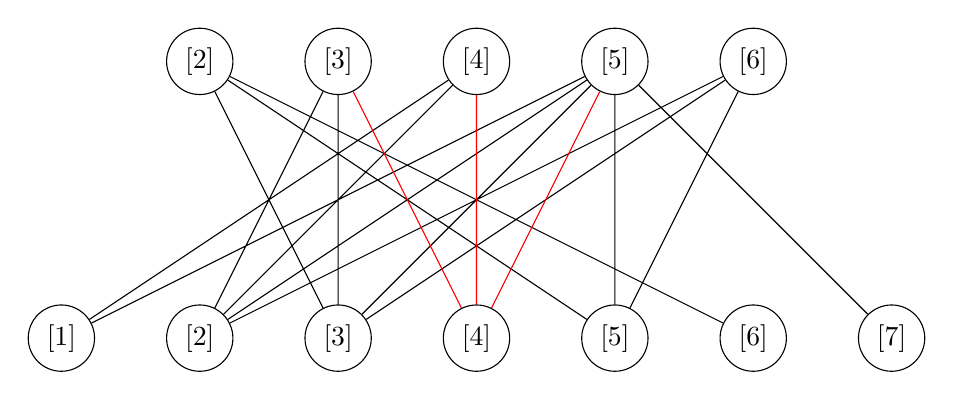
\begin{tikzpicture}
        {\tikzstyle{every node}=[circle, draw]
          \foreach \i in {2, ..., 6}
          {
            \node (s\i) at (\i*50pt, 100pt) {\species[\i]};
          }

          \foreach \j in {1, ..., 7}
          {
            \node (c\j) at (\j*50pt, 0) {\character[\j]};
          }
        }

        \draw
          (c1) -- (s4)
          (c1) -- (s5)
          (c2) -- (s3)
          (c2) -- (s4)
          (c2) -- (s5)
          (c2) -- (s6)
          (c3) -- (s2)
          (c3) -- (s3)
          (c3) -- (s5)
          (c3) -- (s6)
          (c5) -- (s2)
          (c5) -- (s5)
          (c5) -- (s6)
          (c6) -- (s2)
          (c7) -- (s5);

        \draw[red]
          (c4) -- (s3)
          (c4) -- (s4)
          (c4) -- (s5);
      \end{tikzpicture}

    \caption{Red-black graph \grb{}}
    \label{figure:5:a}
  \end{subfigure}

  \bigskip

  \begin{subfigure}[b]{0.98\textwidth}
    \centering
      \begin{tabular}{l | l}
        \character[i] & $S(\character[i])$ \\ \hline
        \character[1] & $\{ \species[4], \species[5] \}$ \\
        \character[2] & $\{ \species[3], \species[4], \species[5], \species[6] \}$ \\
        \character[3] & $\{ \species[2], \species[3], \species[5], \species[6] \}$ \\
        \character[5] & $\{ \species[2], \species[5], \species[6] \}$ \\
        \character[6] & $\{ \species[2] \}$ \\
        \character[7] & $\{ \species[5] \}$
      \end{tabular}

    \caption{Adjacency lists of the inactive characters in \grb{}}
    \label{figure:5:b}
  \end{subfigure}

  \bigskip

  \begin{subfigure}[b]{0.98\textwidth}
    \centering
      {\renewcommand{\arraystretch}{1.5}
      \begin{tabular}{| l | l | l | l |}
        \hline

        \boldmath $S(\character[i])$, $\character[i] \in \grb{}$ &
        \boldmath $S(\character[j])$, $\character[j] \in \cm{}$ &
        \boldmath $Operation$ &
        \boldmath \cm{} \\

        \hline

        $S(\character[1]) = \{ \species[4], \species[5] \}$ &
        &
        Add \character[1] &
        $\{ \character[1] \}$ \\

        \hline

        $S(\character[2]) = \{ \species[3], \species[4], \species[5], \species[6] \}$ &
        $S(\character[1]) = \{ \species[4], \species[5] \}$ &
        Replace \character[1] &
        $\{ \character[2] \}$ \\

        \hline

        $S(\character[3]) = \{ \species[2], \species[3], \species[5], \species[6] \}$ &
        $S(\character[2]) = \{ \species[3], \species[4], \species[5], \species[6] \}$ &
        Add \character[3] &
        $\{ \character[2], \character[3] \}$ \\

        \hline

        $S(\character[5]) = \{ \species[2], \species[5], \species[6] \}$ &
        $S(\character[2]) = \{ \species[3], \species[4], \species[5], \species[6] \}$ &
        &
        \\

        &
        $S(\character[3]) = \{ \species[2], \species[3], \species[5], \species[6] \}$ &
        Ignore \character[5] &
        $\{ \character[2], \character[3] \}$ \\

        \hline

        $S(\character[6]) = \{ \species[2] \}$ &
        $S(\character[2]) = \{ \species[3], \species[4], \species[5], \species[6] \}$ &
        &
        \\

        &
        $S(\character[3]) = \{ \species[2], \species[3], \species[5], \species[6] \}$ &
        Ignore \character[6] &
        $\{ \character[2], \character[3] \}$ \\

        \hline

        $S(\character[7]) = \{ \species[5] \}$ &
        $S(\character[2]) = \{ \species[3], \species[4], \species[5], \species[6] \}$ &
        Ignore \character[7] &
        $\{ \character[2], \character[3] \}$ \\

        \hline
      \end{tabular}}

    \caption{Computation of \cm{} for \grb{}}
    \label{figure:5:c}
  \end{subfigure}


  \caption{Process of computing the set of maximal characters \cm{} for a red-black graph \grb{}}\label{figure:5}
\end{figure}

\pagebreak

\subsubsection{HDGraph class}\label{section:hdgraph-class}

The Hasse diagram class implements a directed acyclic graph with labeled edges.
\wip{Continue}

\subsubsection*{Traits and properties}

\todo[inline]{Add introduction?}

\begin{lstlisting}[belowskip=0pt]
  typedef boost::adjacency_list<
    boost::setS,           // OutEdgeList
    boost::vecS,           // VertexList
    boost::bidirectionalS, // Directed
    HDVertexProperties,    // VertexProperties
    HDEdgeProperties,      // EdgeProperties
    HDGraphProperties      // GraphProperties
  > HDGraph;
\end{lstlisting}

\paragraph{OutEdgeList}

Set to !boost::setS!, because we couldn't notice any performance losses caused by using a set instead of a list or vector, unlike with our red-black graph class.
This may be caused by the fact that we don't alter the structure of the graph in our algorithms, we just construct and deconstruct it.

So, we opted for keeping !setS!, which enforces our Hasse diagram to have at most one edge between two vertices.

We propose another benchmark comparing runtimes of the program. In input, the three $320 \times 320$ PPP instances we tested before:

\begin{center}
  \begin{tabular}{c | c c c c}
    $Instance$ & $setS$   & $listS$  & $slistS$ & $vecS$ \\
    \hline
    Instance 0 & $13.28s$ & $13.39s$ & $13.45s$ & $13.34s$ \\
    Instance 1 & $41.73s$ & $42.05s$ & $42.14s$ & $42.05s$ \\
    Instance 2 & $45.25s$ & $45.56s$ & $45.78s$ & $45.83s$
  \end{tabular}
\end{center}

\paragraph{VertexList}

Set to !boost::vecS!, so we don't have to build the index map of the vertices when calling a Boost function that requires the graph to have indexed vertices.
Furthermore, when the operations performed on a Boost Graph don't involve the deletion of vertices, there is no reason not to use !vecS! as underlying data structure.

\paragraph{Directed}

Set to !boost::bidirectionalS!, as opposed to !directedS!, so that we could make use of the Boost function !in_edges! to perform a simple transitive reduction of the Hasse diagram during its construction.

\paragraph{VertexProperties}

Set to !HDVertexProperties!, i.e., the struct that characterizes a vertex in the Hasse diagram.

\begin{lstlisting}
  struct HDVertexProperties {
    std::list<std::string> species;
    std::list<std::string> characters;
  };
\end{lstlisting}

Each vertex in the Hasse diagram is labeled by a set of species which share the same characters; this is represented with the struct shown in the snippet above, which stores lists of species and a character names (strings).

Storing strings instead of !RBVertex! for identifying vertices may not be the most elegant solution, however, the choices were limited.
While the Hasse diagram represents the poset $(P_{s}, \leq)$ of the species of a graph \grbcm{}, if we stored the vertices as !RBVertex! descriptors of the graph \grbcm{} we would lose direct access to the !RBVertex! descriptor of the original \grb{}.
This is because \grbcm{} is a copy of the graph \grb{}, not a filtered view, and copies mean different descriptors (with !slistS! as vertex container).

Summarizing, we store vertex names in !HDVertexProperties! \textendash{} with the support of the previously introduced !bimap! \textendash{} to render constant-time access (random access) feasible from a species (character) in a !HDVertex! to its respective species (character) in \grb{} and \grbcm{}.

\paragraph{EdgeProperties}

Set to !HDEdgeProperties!, which we define as a list of signed (positive) characters.

\begin{lstlisting}[moreemph={SignedCharacter}]
  struct HDEdgeProperties {
    std::list<SignedCharacter> signedcharacters;
  };
\end{lstlisting}

Each edge \edge{v_{i}}{v_{j}} in a Hasse diagram for a graph \gm{} is labeled by the set of positive characters that are present in $v_{j}$ and not in $v_{i}$.
We represent this set as a list of signed characters. A signed character is structured as follows:

\begin{lstlisting}[belowskip=0pt, moreemph={State}]
  struct SignedCharacter {
    std::string character;
    State state;
  };
\end{lstlisting}

Character vertices are stored in a signed character as strings \textendash{} vertex names \textendash{} like in !HDVertexProperties!.

Finally, the scoped enumeration indicating the type of !state! is stored as such:

\begin{lstlisting}[belowskip=0pt]
  enum class State : bool {
    lose,
    gain
  };
\end{lstlisting}

Signed characters labeled as \character[][-] are associated with a state !State::lose!, while the state of signed characters \character[][+] is !State::gain!.

\paragraph{GraphProperties}

Set to !HDGraphProperties!, that we use to store pointers to the \grb{} and \gm{} graphs associated with the Hasse diagram.

\begin{lstlisting}[moreemph={RBGraph}]
  struct HDGraphProperties {
    const RBGraph* g;
    const RBGraph* gm;
  };
\end{lstlisting}

The pointers are non-const since we need to be able to initialize them using a simple assignment.
We provide functions for accessing !g! and !gm! that support pointer constness:

\begin{lstlisting}[belowskip=0pt, moreemph={RBGraph, HDGraph},
                   moreemph={[2]orig_g}]
  const RBGraph* const orig_g(const HDGraph& hasse);
\end{lstlisting}

\begin{lstlisting}[aboveskip=\smallskipamount, moreemph={RBGraph, HDGraph},
                   moreemph={[2]orig_gm}]
  const RBGraph* const orig_gm(const HDGraph& hasse);
\end{lstlisting}

The red-black graphs stored in Hasse diagram's GraphProperties allow us to have one-to-one correspondences between the vertex names stored in the diagram and the species and characters of the original graphs.

\subsubsection*{General purpose functions}

The overloaded output stream operator for a !HDGraph! prints the adjacency lists of each vertex in the diagram, showing all the informations stored in the VertexProperties and EdgeProperties.

The diagram of figure \ref{figure:4:b}, printed with the ostream operator:

\begin{lstlisting}[belowskip=0pt, keywordstyle=\color{block_fg}]
  [ s0 ( c2 ) ]: -c3+-> [ s5 ( c2 c3 ) ];
  [ s1 s2 ( c1 ) ]: -c3+-> [ s4 ( c1 c3 ) ];
  [ s4 ( c1 c3 ) ]: -c2+-> [ s3 ( c1 c2 c3 ) ];
  [ s5 ( c2 c3 ) ]: -c1+-> [ s3 ( c1 c2 c3 ) ];
  [ s3 ( c1 c2 c3 ) ]:
\end{lstlisting}

\subsubsection*{Algorithm functions}

\todo[inline]{Add introduction?}

\paragraph{Hasse diagram}

To build the Hasse diagram of a maximal reducible graph \gm{}, we start by preparing an array of species of \gm{} sorted in ascending order by the number of characters adjacent to them.

Then, for each species \species[i], we draw up its list of adjacent character names and, if a !HDVertex! $v_{j}$ with the same characters already exists, we append \species[i] to the list of species of $v_{j}$. Otherwise, we add a new !HDVertex! labeled by \species[i] and its list of adjacent characters.

Every time a new !HDVertex! $v_{i}$ is added in the Hasse diagram, we build new edges from the other vertices $v_{j}$ to the vertex $v_{i}$ when needed, i.e., the set of characters of $v_{j}$ is included in the set of characters of $v_{i}$.

The last step involves performing a transitive reduction on the diagram, since many edges may be connecting two vertices $v_{i}$ and $v_{j}$, while a path $v_{i} \rightarrow v_{k} \rightarrow v_{j}$ already exists.

\subsection{Algorithm functions}\label{section:algorithm-functions}

\todo[inline]{Add introduction?}

\subsubsection{Realize characters and species}\label{section:realize}

Multiple definitions for the Realize function have been implemented in the project; these definitions differ from each other by the first argument's type of the function.

The functions return the list of realized signed characters paired with a boolean value. The boolean will be True if the realization of the first argument is feasible for the graph; conversely, the boolean will evaluate to False if the realization is not feasible, and the list of realized characters produced in output will be empty.

\text{} % keep or not?

\begin{lstlisting}[moreemph={RBGraph, SignedCharacter},
                   moreemph={[2]realize}]
  std::pair<std::list<SignedCharacter>, bool>
  realize(const SignedCharacter& sc, RBGraph& g);
\end{lstlisting}

The first definition concerns the realization of a single signed character \character[][\pm] (!sc!) in a graph \grb{} (!g!).

Before realizing a character we compute the connected components of the graph and verify whether the character in input is inactive and positive (\character[][+]) or active and negative (\character[][-]). When running the Reduce function, no realization should be non-feasible.

Characters in the graph may become free or universal following the realization of the signed character !sc!.
Making sure to realize free and universal characters whenever possible is critical to the correctness of the algorithm.

\text{} % keep or not?

\begin{lstlisting}[moreemph={RBGraph, SignedCharacter},
                   moreemph={[2]realize}]
  std::pair<std::list<SignedCharacter>, bool>
  realize(const std::list<SignedCharacter>& lsc,
          RBGraph& g);
\end{lstlisting}

An extension of the previously discussed definition involves the realization of a sequence of signed characters. In our implementation, we define this sequence as a list of signed characters \character[][\pm] (!lsc!).

Since the Realize function for realizing a each signed character may perform multiple realizations (free and universal characters), we had to introduce a check to verify that the next signed character that we want to realize hasn't already been realized.

\text{} % keep or not?

\begin{lstlisting}[moreemph={RBGraph, SignedCharacter, RBVertex},
                   moreemph={[2]realize}]
  std::pair<std::list<SignedCharacter>, bool>
  realize(const RBVertex v, RBGraph& g);
\end{lstlisting}

Following the definition \ref{definition:realization} we described the realization of a species \species[i] as the realization of the set of inactive characters adjacent to \species[i].

This function builds the list of positive characters \character[j][+] for the input species \species[i] (!v!), giving it in input, as the first argument, to the other Realize function.

\subsubsection{Find initial state(s)}\label{section:initial-state}

The Find-initial-state procedure described in algorithm \ref{algorithm:find-initial-state} computes a safe source of a Hasse diagram (if it exists), however, to support the command line arguments introduced in the previous sections, we adjusted the algorithm to be able to return multiple safe sources; then, the function to obtain the initial state(s) returns a list of !HDVertex!.

Finding chains in the Hasse diagram is performed by calling the Boost function for depth-first search; this function invokes user-defined actions at certain event-points within the algorithm.
These actions are defined inside a visitor class.
The DFS Visitor we implemented derives from the default DFS Visitor:

\begin{lstlisting}
  class initial_state_visitor : public boost::default_dfs_visitor
\end{lstlisting}

The Initial state visitor implements the set of visitor functions with the intent of finding a safe chain and testing whether the source of the chain passes the Test 1 (line \ref{algorithm:find-initial-state:test1} of Find-initial-state).
If Test 1 succeds, we add the source to the list of safe sources; otherwise, we add it to the list of feasible sources.

When running the polynomial-time version of the algorithm, a custom !InitialState! exception is thrown from the visitor whenever a source passes Test 1.
This is considered standard practice in Boost when performing an early exit from an algorithm.

If at the end of DFS visit the list of safe sources is empty, we proceed with Tests 2 and 3 (line \ref{algorithm:find-initial-state:test2} and \ref{algorithm:find-initial-state:test3}), as described in the Find-initial-state procedure.

We noticed some problems with this approach.
The standard implementation of a DFS algorithm colors "finished" vertices in black; however, when building a chain in the diagram, it might happen that the chain includes finished vertices.
We built a temporary workaround to this, which will soon be replaced with a more appropriate function.

\subsubsection{Reduce}\label{section:reduce}

The Reduce function returns a list of !SignedCharacter!, where each signed character represents a realization performed by the algorithm.

A custom !NoReduction! exception is thrown by the function if the computed Hasse diagram doesn't have any safe sources.
Being the implementation recursive, this proved to be the simplest way of exiting the program.

Support for the command line arguments has been implemented in the function.
The exponential version of the algorithm realizes the safe sources in a recursive depth-first manner.
The interactive option makes the algorithm stop and wait for the user to select a source from the list of safe sources found in the Hasse diagram.
In the polynomial-time version the first (and only) safe source is realized, however, with the $N$th source option, the realized source tries to reflect the choice selected in the argument.

One last thing to note: when appending the list of realized characters to the output, we do so in constant time by using the !std::list::splice! function, which doesn't copy the data unnecessarily.

E.g., this is how we implemented the concatenation of multiple Reduce calls on the connected components of the graph (!output! is the list of signed characters, !g! is the red-black graph):

\begin{lstlisting}[moreemph={RBGraphVector, RBGraph}]
  RBGraphVector comps = connected_components(g);

  if (comps.size() > 1) {
    for (const std::unique_ptr<RBGraph>& comp : comps) {
      output.splice(output.cend(), reduce(*comp.get()));
    }

    return output;
  }
\end{lstlisting}
